% !TeX root=../main.tex
\chapter{موقعیت‌یابی و کالیبراسیون به صورت همزمان یک ربات کابلی با در نظر گرفتن کابل‌ها به صورت جسم صلب}

\section{مقدمه}
همانطور که در فصل قبل ذکر شد، اگرچه سنسورهای فضای مفصل سریع و ارزان هستند، اما زمانی که از آنها برای اندازه‌گیری مقادیر مجری نهایی استفاده می‌شود، دقت مدل  سینماتیکی برای تعیین دقت قابل دستیابی بسیار مهم است. 
علاوه بر این، در زمینه همجوشی و ترکیب اندازه‌گیری‌ها، هم‌ثبت کردن داده ها \cite{hall1997introduction} اولین گام اساسی است. به عبارت دیگر، حسگرها باید اندازه‌گیری‌های خود را در یک مختصات یکپارچه ارائه دهند. اهمیت هم‌ثبت به دلیل فرض اساسی نویز گاوسی با میانگین صفر در الگوریتم‌های ترکیب داده‌ها می باشد. 
نکته قابل توجه دیگر برای ربات های آسان نصب، لزوم بی نیازی الگوریتم کالیبراسیون پیشنهادی به حسگرهای گران  قیمت و یا حسگرهایی که نیاز به تعمیر و نگهداری سطح بالایی هستند می باشد. علاوه بر این، فرآیند کالیبراسیون باید به اندازه‌ای ساده باشد که اجرای آن در مکان‌های مختلف آسان و سریع باشد.  
با اینکه کالیبراسیون موضوعی است که بسیاری از پژوهشگران به آن علاقه‌مند هستند، اما مفهوم بهره‌گیری از چندین حسگر برای بهبود نتایج کمتر مورد توجه قرار گرفته است. علاوه بر این، الگوریتم کالیبراسیون یکپارچه و قابل گسترش در ادبیات برای ربات‌های کابلی وجود ندارد. 

از طرفی دیگر، افزون بر مفهوم و ضرورت کالیبراسیون در این ربات ها، موقیت یابی این ربات ها نیز مورد توجه بسیاری قرار گرفته است. 
همانطور که پیش تر بیان شد، الگوریتم های بسیاری در راستای ترکیب حسگرها و همچنین کاهش زمان پردازش برای موقعیت یابی ربات به صورت زمان-واقعی در انواع دیگر ربات ها همچون ربات های خودران مورد استفاده قرار گرفته است. 

آنچه در ادامه این رساله مورد توجه قرار می گیرد، آدرس دهی جامع برای حل تمامی موارد بیان شده در بالا می باشد. بدین منظور، رویکردی معرفی می شود که در وهله اول مسائل کالیبراسیون و موقعیت یابی را به صورت یک مسئله یکپارچه در یک قاب ببیند و سپس انعطاف پذیری الگوریتم مجال افزودن حسگرهای اضافی را فراهم نماید. چنین رویکردی نه تنها انجام دو فرآیند مجزای کالیبراسیون و موقعیت یابی را به یک فرآیند ترکیب شده و همزمان تبدیل می کند، بلکه به راحتی می تواند به دیگر الگوریتم های ادبیات موضوع افزوده شود. نتیجه این رویکرد علاوه بر افزایش دقت نهایی این فرآیندها، مفهومی حقیقی تر به آسان نصب بودن به این دسته از ربات های کابلی می بخشد. الگوریتم پیشنهادی برای فرمول بندی این مسئله با آدرس دهی آنچه مورد نیاز ما است، الگوریتم گراف عامل می باشد. ویژگی های منحصر به فرد این الگوریتم در حل مسائل تنک مانند مسئله موقعیت یابی و نقشه برداری به صورت بر خط باعث استفاده زیادی از این فرمول بندی برای طیف وسعی از کاربرد های رباتیکی در سال های اخیر شده است.

در این فصل حل مسئله موقیت یابی و کالیبراسیون به صورت هزمان برای یک ربات کابلی فروتحریک با در نظر گرفتن فرض اساسی صلب بودن کابل ها مورد بررسی قرار می گیرد. در حالی که فرمول بندی مسئله با در نظر گرفتن این فرض بسیار ساده تر می شود، تا زمانی که شکم دهی کابل ها ناشی از جرم آنها بسیار ناچیز باشد، قابل قبول خواهد بود. حل این مسئله برای کابل شکم دار منجر به ایجاد چالش هایی می گردد که در فصل آتی به صورت مفصل به آنها پرداخته می شود و در نهایت با رویکرد پیشنهادی بار دیگر حل می گردد. 

\subsection{روش های مرسوم مسئله کالیبراسیون} \label{seq:conventional_calibration}
به صورت کلی، انتظار می رود چنانچه به یک ربات در دنیای واقع یک ورودی مشخص اعمال شود، با اعمال همان ورودی به مدل پاسخی یکسان دریافت شود. با این حال همواره وجود نامعینی ها و عدم دقیق بودن پارامتر های مدل در واقعیت ما را از رسیدن به چنین پاسخی ایده آل باز می دارد. این نامعینی ها می تواند ناشی از تقریب هایی باشد که در مدل داریم و یا پدیده هایی که در مدل سازی مورد توجه کامل قرار نگرفته اند. جنس این نامعینی ها می تواند ریشه در سینماتیک ربات و یا دینامیک آن باشد. فرآیند کالیبراسیون می تواند این نامعینی ها را در جهتی کاهش دهد که پاسخ هایی که از مدل و ربات در پیاده سازی واقعی دریافت می کنیم، کاهش پیدا کند. آنچه در این کار مورد بررسی قرار گرفته است کالیبراسیون سینماتیکی می باشد. شکل \ref{fig:kinematicmodelerror} نمایش بلوکی از یک فرآیند کالیبراسیون سینماتیکی بنا بر تعریف بیان شده می باشد. همانطور که در این شکل مشاهده می شود آنچه به عنوان خطا در نظر گرفته می شود تفاوت موقعیت فضایی ربات است که ناشی از مدل سینماتیکی ربات (در اینجا سیتماتیک مستقیم) و ربات واقعی در فضای کاری ربات، با یک ورودی مشترک در فضای مفصلی آن می باشد. 

\begin{figure}[!t]
	\centering
	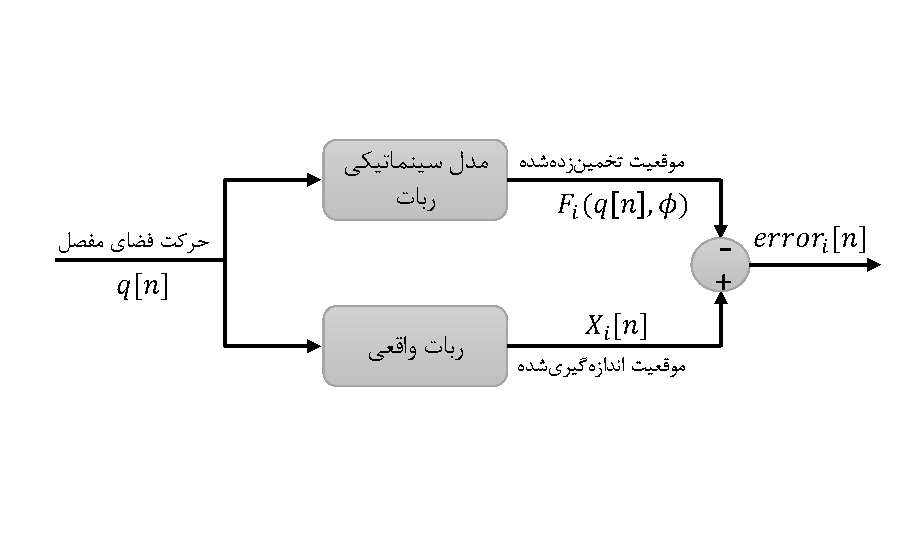
\includegraphics[width=0.8\linewidth, trim={0cm 2.2cm 0cm 2.2cm}, clip]{img/kinematic_model_error}
	\caption{}
	\label{fig:kinematicmodelerror}
\end{figure}


با نگاهی به آخرین تحقیقات بر روی مسئله کالیبراسیون ربات ها، ایجاد یک مسئله بهینه سازی غیرخطی و حل آن برای یافتن مقادیر دقیق این پارامتر های سینماتیکی و دینامیکی ربات مرسوم می باشد
\cite{elatta2004overview,ida2019automatic,ida2022identification,ida2021dynamics}.
مطابق این رویکرد های مروسم، برای ایجاد فرمول بندی مناسب مسئله مطرح شده در شکل \ref{fig:kinematicmodelerror} خواهیم داشت:

\begin{equation}\label{eq:optimization_equation_conventional}
	\tilde{\boldsymbol{\phi}} =  \arg\min_{\boldsymbol{\phi}} \sum_{n = 1 }^{N} \text{error}_i[n] = \arg\min_{\boldsymbol{\phi}} \sum_{n = 1}^{N} ||F_i(\boldsymbol{q}[n], \boldsymbol{\phi}) - X_i[n]||^2_{\Sigma}
\end{equation}

در این معادله، $\boldsymbol{\phi}$ بردار پارامتر های سینماتیکی و $\tilde{\boldsymbol{\phi}}$ تخمین آن است. علاوه بر این، $X_i[n]$، 
$iامین$
مقدار اندازه گیری شده توسط حسگر فضای کار ربات، و $\boldsymbol{q}[.]$ مقادیر اندازه گیری های متقابل حسگری در مفاصل می باشد. تابع مدل ربات $F[.]$ بیانگر مدل سینماتیک مستقیم ربات می باشد. تابع هزینه هدف، بر روی مجموعی از $N$ نمونه داده جمع آوری شده در فرآیند کالیبراسیون می باشد. افزون بر این، $\Sigma$ نیز بیانگر ماتریس کوواریانس اندازه گیری می باشد که به عنوان عامل نرمال سازی برای محاسبه هزینه عمل می کند. هر چه مقدار کوواریانس بیشتر باشد، میزان تاثیر گذاری خطای متقابل آن بر روی تابع هزینه کمتر خواهد بود. همچنین برای محاسبه نرم روش های زیادی ارائه شده است که آنچه بیشتر مورد استفاده قرار می گیرد نرم های هابر 
\footnote{\lr{Huber norms}}
می باشد
\cite{chang2015huber}.
معادله بهینه سازی غیر خطی بیان شده در 
\ref{eq:optimization_equation_conventional}
می تواند با روش های بازگشتی الگوریتم های غیر خطی حداقل مربعات
\footnote{\lr{Least-Square}}
همچون  لونبرگ-مارکوارت
\footnote{\lr{Levenberg Marquardt (LM)}}
و یا روش های گاوس-نیوتون
\footnote{\lr{Gauss-Newton(GN)}}
می باشد
\cite{dellart_robot_perception}.

با نگاهی دیگر به دیاگرام مطرح شده در 
\ref{fig:kinematicmodelerror}
و همچنین معادله 
\ref{eq:optimization_equation_conventional}،
مشاهده می‌شود که افزایش دقت اندازه‌گیری و همچنین برآورده کردن تمامی قیود مدل می‌تواند منجر به بهبود نتیجه کالیبراسیون شود. به منظور دستیابی به این هدف، رویکردهایی همچون ترکیب چندین حسگر و یا افزودن قیود جدید که از ساختار هندسی ربات استخراج می‌شود، معرفی می‌شوند. ترکیب این حسگرها باید به گونه‌ای باشد که علاوه بر کاهش خطای نهایی کالیبراسیون، خروج هر کدام از حسگرها منجر به توقف فرآیند کالیبراسیون نشود. همچنین واضح است که افزودن این قیود می‌تواند منجر به حل پیچیده‌تری از مسئله شود. در ادامه، نگاهی به فرمول‌بندی مسئله کالیبراسیون با در نظر گرفتن این ترکیب‌ها خواهیم داشت.

\subsubsection{ترکیب حسگر ها}
در معادله 
\ref{eq:optimization_equation_conventional}،
زیرنویس 
$i$
بیانگر وجود یک حسگر و خطایی که از مقادیر اندازه گیری حسگر در هر نمونه بوده می باشد. فرمول بندی ساختاری که به صورت همزمان از چندین حسگر در راستای ایجاد تابع هزینه استفاده نماید می تواند به صورت زیر تعریف شود:
\begin{equation}\label{eq:optimization_equation_conventional_multi_sensor}
	\tilde{\boldsymbol{\phi}} =  \arg\min_{\boldsymbol{\phi}} \sum_{n = 1 }^{N} \sum_{n = 1 }^{M} W_i~\text{error}_i[n] 
\end{equation}
در این معادله 
$W_i$
ها یک پارامتر وزن برای ترکیب چندین منبع اطلاعاتی با توجه به میزان کیفیت و اهمیت آنها می باشد.


\subsubsection{ترکیب شبه اندازه گیری ها}
اندازه گیری های حسگری تنها منبع اطلاعات برای حل مسئله نیستند. ساختار ربات و توحه به هندسه آن برای حل مسئله تعریف شده می تواند مفید واقع شود. برای مثال فاصله های بین برخی از نقاط می تواند با توجه به ساختار ربات می توانند ویژگی هایی نسبی و یا مطلق داشته باشند. این اطلاعات با عنوان داده های شبه اندازه گیری شناخته می شوند. این دسته از اطلاعات که از قبل مشخص هستند، می توانند به صورت قیود به مسئله اضافه شوند. بنابراین مسئله کلی بهینه سازی کالیبراسیون
\ref{eq:optimization_equation_conventional_multi_sensor}
در حضور این قیود به صورت زیر باز نویسی می شود. 
\begin{equation}
	\begin{aligned}
		&\tilde{\boldsymbol{\phi}} =  \arg\min_{\boldsymbol{\phi}} \sum_{n = 1 }^{N} \sum_{n = 1 }^{M} W_i~\text{error}_i[n] \\
		\quad &g_j(\boldsymbol{\phi}) = 0 \quad where \quad j = 1, \ldots, K
	\end{aligned}
\end{equation}
که در اینجا
$g_j(\boldsymbol{\phi}) = 0$ 
قیود هندسی معلوم بر روی پارامترهای سینماتیکی ربات می باشند.

\subsection{روش های مرسوم مسئله موقعیت یابی}
موقعیت یابی
\footnote{Localization}
 ربات فرآیند تعیین مکان ربات نسبت به محیط اطراف آن می باشد. دانستن موقعیت دقیق ربات در محیط، پیش‌نیازی اساسی برای اتخاذ تصمیمات صحیح و حرکت های بعدی مؤثر است. بدون اطلاعات موقعیتی دقیق، ربات نمی‌تواند مسیریابی
\footnote{motion planing}
  و یا ردیابی
\footnote{trakcing}
مناسبی را داشته باشد و ممکن است با موانع برخورد کند یا مسیر بهینه‌ای را طی نکند
\cite{ahmad2013cooperative}.
 علاوه بر این، سیستم‌های کنترلی ربات‌ها نیازمند اطلاعات دقیق و لحظه‌ای از موقعیت و جهت‌گیری ربات هستند تا بتوانند فرمان‌های مناسب را صادر کنند. بدون داده‌های دقیق موقعیتی، کنترلرها نمی‌توانند حرکات دقیقی را تولید کنند که منجر به عملکرد نامناسب و ناپایداری ربات می‌شود
\cite{guibas1997robot}.
فرآیند کالیبراسیون ربات که در بخش 
\ref{seq:conventional_calibration}
مورد بررسی قرار گرفت نیز یازمند داشتن اطلاعات دقیق از موقعیت ربات است. با داشتن داده‌های موقعیتی دقیق، می‌توان خطاهای سیستماتیک را شناسایی و تصحیح کرد و به این ترتیب دقت و کارایی ربات را بهبود بخشید. این امر به ویژه در ربات‌هایی که نیاز به انجام وظایف حساس و دقیق دارند، حیاتی است. 

موقعیت‌یابی دقیق ربات باعث کاهش عدم قطعیت در تصمیم‌گیری‌ها و عملیات ربات می‌شود. این امر نه تنها به افزایش اعتمادپذیری ربات در انجام وظایف محوله منجر می‌شود، بلکه احتمال بروز خطاها و حوادث ناشی از اشتباهات موقعیتی را نیز کاهش می‌دهد. همچنین در سیستم‌هایی که شامل چندین ربات هستند، اطلاعات دقیق موقعیتی هر ربات برای هماهنگی و همکاری بین ربات‌ها ضروری است. این اطلاعات به ربات‌ها کمک می‌کند تا از موقعیت یکدیگر آگاه باشند و بتوانند به صورت هماهنگ وظایف مشترک را انجام دهند. در این راستا توسعه و بهبود تکنیک‌های موقعیت‌یابی به منظور افزایش دقت و کارایی ربات‌ها، از اهمیت ویژه‌ای برخوردار است
\cite{aragues2011multi}.


روش های ارائه شده برای موقعیت یابی ربات را می توان به سه دسته اصلی مسافت پیمایی
\footnote{odometry}،
موقعیت یابی جهانی
\footnote{global localization}
و مکان یابی و نقشه یابی به صورت همزمان
\footnote{SLAM}
تقسیم کرد. این روش ها با توجه به نوع حسگرهای تعبیه شده بر روی ربات می تواند مورد استفاده قرار گیرد. ترکیب داده ها برای همانند آنچه در بخش
\ref{seq:conventional_calibration}
مورد توجه قرار گرفت، در موقعیت یابی و تخمین حالت ربات نیز می تواند نقش موثری را ایفا کند. حسگر های استفاده شده از نظر نوع حسگر و فرکانس داده برداری نیز می تواند متفاوت باشد که در ترکیب داده ها خصوصا زمانی که اجرای الگوریتم به صورت زمان واقعی می باشد، چالش برانگیز خواهد بود. طیف وسیعی از روش های مرسوم ارائه شده برای ترکیب داده ها در راستای تخمین حالت، رویکرد های بر مبنای فیلتر هستند. این روش ها که به رویکرهای آماری 
\footnote{stochastic}
نیز شناخته می شوند، در دو دهه اخیر فعالیت های زیادی را به خود اختصاص داده اند. پایه این روش ها بر قانون بیز
\footnote{Bayes law}
بنا نهاده شده است. 
\cite{panigrahi2022localization} 
دسته بندی جامعی از روش های فیلتر مبنا برای تخمین موقعیت ارائه کرده است. از میان روش های بیان شده، کالمن فیلتر و فیلترهای ذرات
\footnote{particle filters}
به عنوان فراگیرترین رویکرد مورد استفاده قرار گرفته شده است. این فیلترها با استفاده از فرض مارکووی برای حالت ها و به کار گیری اطلاعات پیشین، تخمینی از حالت جدید ارائه می کنند. 






 
 
 
 
 
 
 
 
 
 
 
 
 
 
 